\documentclass{article}

\usepackage{amsmath,graphicx,array}

\title{High MSWDs are not the problem, low ones are\\}

\author{Pieter Vermeesch \\ Department of Earth Sciences \\ University College London}

\begin{document}

\maketitle

The Mean Square Weighted Deviation (MSWD) is a widely used measure of
statistical dispersion in geochronology.  It quantifies the degree to
which analytical uncertainty explains the observed scatter of some
data around a weighted mean or regression
line\cite{mcintyre1966}. There is a misconception among some
geochronologists that low MSWD values are `good' and that high MSWD
values are `bad'. This attitude is misguided.

\begin{itemize}
  \item Overdispersed datasets are not the exception but the rule in
    geochronology.
  \item The absence of excess dispersion in geochronological datasets
    should raise suspicion, not praise.
  \item Dispersion should not be feared but quantified.
\end{itemize}

To illustrate these points, consider a collection of $n$ igneous
zircon crystals, and let $\{t_1,\ldots{t_i},\ldots,t_n\}$ be their
true ages. Compare the following two scenarios:

\begin{description}
\item{Scenario~1}: the zircons all formed at exactly the same time
  $t$, so that $t_i=t$ for all $1\leq{i}\leq{n}$.
\item{Scenario~2}: the zircons formed over a finite time interval, so
  that ${t_i}\neq{t_j}$ if ${i}\neq{j}$.
\end{description}

The true ages $t_i$ are unknown but can be estimated from isotopic
data. Let $\hat{t}_i$ be the measured \emph{date} of the
$i$\textsuperscript{th} zircon crystal, and let $\sigma_i$ be its
known analytical uncertainty. Assume that $\hat{t}_i$ was drawn from a
normal distribution with mean $t_i$ and standard deviation $\sigma_i$.

Under Scenario~1, the true zircon formation age $t$ can be estimated
(as $\bar{t}$) by taking the weighted mean of the measured dates:
\begin{equation}
  \bar{t} = \frac{\sum_{i=1}^n\hat{t}_i/\sigma_i^2}{\sum_{i=1}^n1/\sigma_i^2}
  \label{eq:tbar}
\end{equation}

The weighted mean can be misleading under Scenario~2. For example, if
the true ages follow a bimodal distribution, then the weighted mean
date would fall between the two modes.  It is, therefore, of
considerable interest to differentiate between Scenarios~1 and 2. The
MSWD offers a way to do this.  The MSWD of the weighted mean is
defined as follows:
\begin{equation}
  \mbox{MSWD} = \frac{1}{d\!f}\sum_{i=1}^n\left(\frac{\hat{t}_i-\bar{t}}{\sigma_i}\right)^2
  \label{eq:MSWD-wtdmean}
\end{equation}

\noindent where $d\!f$ is the number of `degrees of freedom'
($d\!f=n-1$). Note that, if $\sigma_i=1$ for all $i$, then
Equation~\ref{eq:MSWD-wtdmean} is identical to the sample variance.
Scenario~1 is rejected in favour of Scenario~2 if
$\mbox{MSWD}>1+2\sqrt{2/d\!f}$ (at a 95\% confidence level, provided
that $d\!f>3$ \cite{wendt1991}).  Importantly, low
($\mbox{MSWD}<1+2\sqrt{2/d\!f}$) values do \emph{not} mean that
Scenario~1 is \emph{accepted}. In statistics, as in science in
general, hypotheses cannot be proved. They can only disproved.

There are four possible outcomes for the MSWD-test: Scenario~1 may be
true or false, and MSWD may be below or above the cutoff. There are
two ways to make a correct decision, and two ways to make a
mistake. The mistakes are known as Type-I and Type-II errors:

\begin{description}
  \item{Type-I errors (false positives) are committed when Scenario~1
    is true but the MSWD exceeds the critical value. Their probability
    of occurrence is usually referred to as $\alpha$. If the
    $1+2\sqrt{2/d\!f}$ MSWD cutoff is used, then $\alpha\approx{0.05}$.}
  \item{Type-II errors (false negatives) are committed when Scenario~1
    is false but the MSWD is below the critical value. Their probability
    of occurrence is referred to as $\beta$. The probability $1-\beta$
    is also known as the \emph{power} of a statistical
    test\cite{cohen1992}.}
\end{description}

Figure~\ref{fig:MSWD} illustrates these important concepts using six
synthetic datasets from three idealised hypothetical samples.

The first row of Figure~\ref{fig:MSWD} (panels a--c) shows the true
age distributions of the three samples.  The first sample (panel~a)
follows Scenario~1 with $t=100$\,Ma.  The second sample (panel~b)
follows Scenario~2 for a normal age distribution with mean
$\mu=100$\,Ma and standard deviation $\omega=1$\,Ma. Finally, the
third sample (panel~c) follows Scenario~2 for a normal age
distribution with mean $\mu=100$\,Ma and standard deviation
$\omega=2$\,Ma.

The second row of Figure~\ref{fig:MSWD} (panels d--f), shows three
random samples of $n=10$ dates. For the sake of simplicity, these
dates have a fixed analytical uncertainty of 1\,Ma (i.e.,
$\sigma_i=\sigma=1$\,Ma for all $i$). The third row of
Figure~\ref{fig:MSWD} (panels g--i) shows a further three samples from
the same distributions and with the same analytical uncertainty, but a
larger sample size ($n=50$). The two sample sizes correspond to
slightly different MSWD cutoffs of 1.943 (for $n=10$) and 1.404 (for
$n=50$), respectively.

Comparison of the observed MSWDs with these cutoffs results in six
decisions.  Two of these decisions are wrong. Figure~\ref{fig:MSWD}g
rejects the true Scenario~1, corresponding to a Type-I error, whereas
Figure~\ref{fig:MSWD}e fails to reject the false Scenario~1,
corresponding to a Type-II error. The probability of a Type-I error is
fixed at $\alpha=0.05$. In contrast, the probability of a Type-II
error depends on two factors.

The first factor that affects the power of the MSWD-test is the
magnitude of the difference between Scenarios~1 and 2. This is
illustrated by comparison of Scenarios~2a and 2b. Scenario~1
($\omega=0$\,Ma) is more different from Scenario~2b ($\omega=2$\,Ma)
than it is from Scenario~2a ($\omega=1$\,Ma). Consequently, Scenario~1
is more easily rejected for datasets drawn from population~2b than
from population~2a, and the probability of committing a Type-II error
is correspondingly lower. For a sample size of $n=10$, it can be
shown\footnote{If the true ages were drawn from a normal distribution
with standard deviation $\omega$, then $\beta$ is the
$(d\!f+2\sqrt{2\,d\!f})$-quantile of a chi-squared distribution with
$df$ degrees of freedom that has been shifted by a factor
$(\sigma^2+\omega^2)/\sigma^2$.} that $\beta=0.54$ for Scenario~2a
(Figure~\ref{fig:MSWD}f) and $\beta=0.059$ for Scenario~2b
(Figure~\ref{fig:MSWD}i). In other words, the excess dispersion is
54\% likely to remain undetected for Scenario~2a, but only 5.9\% for
Scenario~2b.

The second factor affecting $\beta$ is sample size ($n$): the larger
the sample, the easier it is to detect departures from
Scenario~1. Recall that, under Scenario~2a, the probability of
committing a Type-II error is 54\% if $n=10$. This drops to 5.6\%
($\beta=0.0056$) if $n=50$ (Figure~\ref{fig:MSWD}f). In other words, a
five-fold increase in sample size increases the power to reject
Scenario~1 by nearly a factor of ten. A similar increase in power is
found for Scenario~2b, where the risk of incurring a Type-II error
reduces from $\beta=0.058$ for $n=10$ to a negligible
$\beta=1.5\times{10}^{-7}$ for $n=50$.

The strong dependence of statistical power on sample size means that,
given a large enough sample, even the tiniest departure from
Scenario~1 becomes detectable. This observation is important because
there is a widespread misconception in geochronology that Scenario~1
is desirable and Scenario~2 is not. In reality, the opposite is
true. Scenario~1 assumes that all zircons crystallise at exactly the
same time (i.e., within the same nanosecond). This is clearly
unrealistic. In real geological settings, zircon crystallisation
always spans a finite range of time, as under Scenario~2. Given a
large enough sample or precise enough data, this time span eventually
becomes detectable, resulting in an `unacceptably' high MSWD.

Some have advocated the use of MSWDs as a screening tool to decide
whether dates can be averaged or not\cite{spencer2016}.  In the
context of isochron regression, high-MSWD fits are commonly referred
to as `errorchrons'\cite{brooks1972}, an undeniably pejorative
term. The author is aware of instances where high MSWD datasets were
deemed to be `unpublishable' by reviewers.  High MSWD datasets are
virtually absent from high impact publications.  These negative
connotations may tempt some scientists to `cherry pick' data, by
removing perceived `outliers' until the MSWD is reduced to an
`acceptable' level. Cherry picking is harmful to science. It degrades
the reproducibility of experiments and discards potentially valuable
geological information.

The purpose of this paper is to provide the reader with a
counter-argument against kneejerk rejections of high MSWD datasets.
Dispersion should not be removed but quantified. Under Scenario~2 of
our synthetic zircon example, this means estimating the dispersion
parameter $\omega$. For very high MSWD values ($>20$, say), doing so
can be as simple as taking the standard deviation of the dates. For
lower MSWD values ($1+2\sqrt{2/d\!f}<\mbox{MSWD}<20$) quantifying the
dispersion requires more sophisticated random effects models
\cite{galbraith1993} or Bayesian inversion methods
\cite{keller2018}. These concepts do not only apply to weighted means,
but can also be generalised to isochron regression
\cite{vermeesch2024}.

In the context of zircon dating, the dispersion of U--Pb dates may
quantify the longevity of magma systems \cite{rioux2012}. In
thermochronology, it can be used to estimate the cooling rate of
exhuming rocks \cite{galbraith1993}.  Steady improvements in
analytical precision and throughput across all geochronological
techniques mean that overdispersed datasets will become even more
prevalent in the future. Our ability to quantify dispersion improves
in tandem with these developments, opening new areas of research.

In conclusion: high MSWD datasets are the rule, not the exception.
Publications containing consistently low MSWD datasets should not be
celebrated but approached with a healthy dose of scepticism.

\begin{figure*}[!ht]
  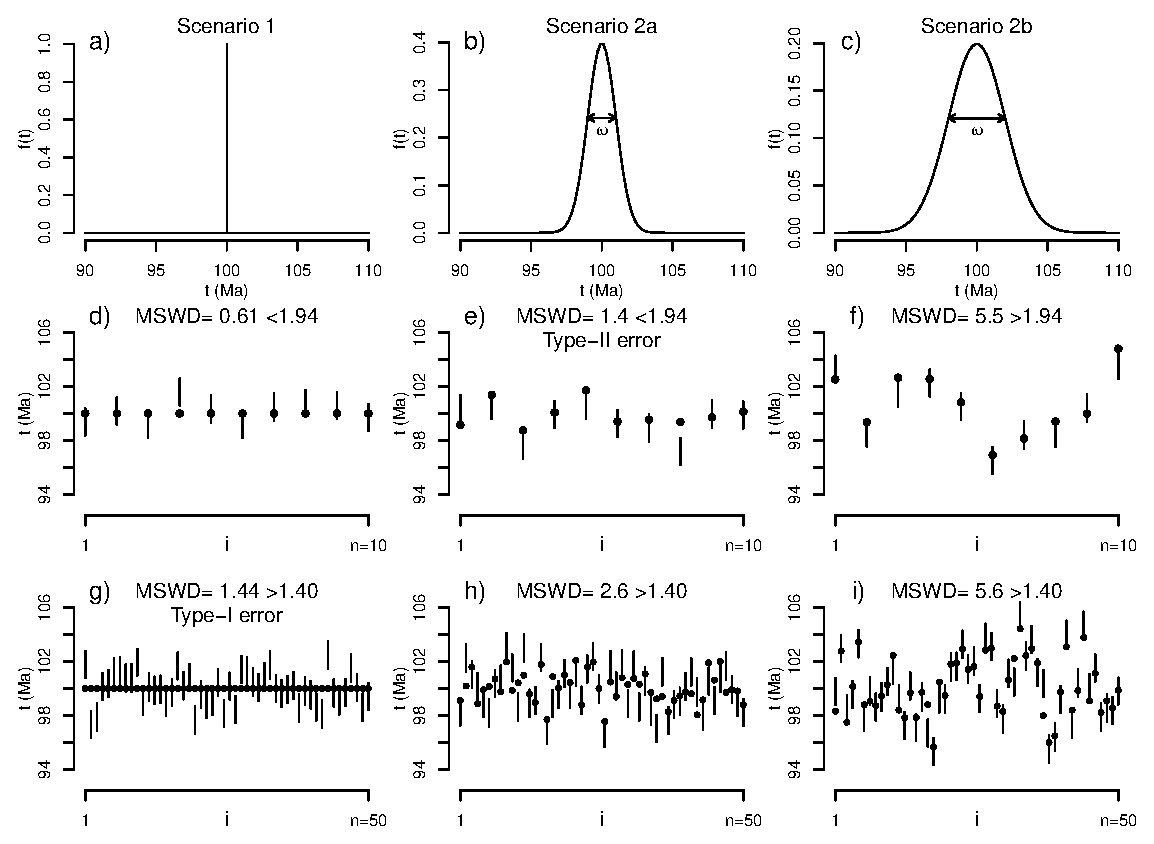
\includegraphics[width=\textwidth]{MSWD.eps}
  \caption{a--c: three hypothetical zircon age distributions, with
    dispersion paramaters $\omega = 0$, 1 and 2\,Ma, respectively;
    d--f: synthetic samples from the three distributions, containing
    $n=10$ dates each (MSWD cutoff $=1.94$); and g--i: three further
    samples with $n=50$ dates each (MSWD cutoff $=1.40$). True ages
    are shown as black circles; measured dates and their uncertainties
    as vertical error bars (shown at $1\sigma$). Comparison of the
    MSWD values with the $1+2\sqrt{2/(n-1)}$ cutoff leads to the
    correct decision in all cases except for panel~e (Type-II error)
    and panel~g (Type-I error).}
  \label{fig:MSWD}
\end{figure*}

%\bibliographystyle{nsr.bst}
%\bibliography{/home/pvermees/Dropbox/biblio.bib}

\begin{thebibliography}{1}

\bibitem{mcintyre1966}
{McIntyre} GA, {Brooks} C, {Compston} W {\em et~al.}
\newblock {The Statistical Assessment of Rb-Sr Isochrons}.
\newblock {\em Journal of Geophysical Research}  1966; {\bf 71}: 5459--5468.

\bibitem{wendt1991}
Wendt I and Carl C.
\newblock The statistical distribution of the mean squared weighted deviation.
\newblock {\em Chemical Geology: Isotope Geoscience Section}  1991; {\bf 86}:
  275--285.

\bibitem{cohen1992}
Cohen J.
\newblock A power primer.
\newblock {\em Psychological bulletin}  1992; {\bf 112}: 155.

\bibitem{spencer2016}
Spencer CJ, Kirkland CL and Taylor RJ.
\newblock {Strategies towards statistically robust interpretations of in situ
  U--Pb zircon geochronology}.
\newblock {\em Geoscience Frontiers}  2016; {\bf 7}: 581--589.

\bibitem{brooks1972}
Brooks C, Hart SR and Wendt I.
\newblock Realistic use of two-error regression treatments as applied to
  rubidium-strontium data.
\newblock {\em Reviews of Geophysics}  1972; {\bf 10}: 551--577.

\bibitem{galbraith1993}
Galbraith RF and Laslett GM.
\newblock Statistical models for mixed fission track ages.
\newblock {\em Nuclear tracks and radiation measurements}  1993; {\bf 21}:
  459--470.

\bibitem{keller2018}
Keller CB, Schoene B and Samperton KM.
\newblock A stochastic sampling approach to zircon eruption age interpretation.
\newblock {\em Geochemical Perspectives Letters}  2018; {\bf 8}.

\bibitem{vermeesch2024}
Vermeesch P.
\newblock {Errorchrons and anchored isochrons in IsoplotR}.
\newblock {\em Geochronology}  2024; {\bf 2024}.

\bibitem{rioux2012}
Rioux M, Lissenberg CJ, McLean NM {\em et~al.}
\newblock {Protracted timescales of lower crustal growth at the fast-spreading
  East Pacific Rise}.
\newblock {\em Nature Geoscience}  2012; {\bf 5}: 275--278.

\end{thebibliography}


\end{document}
